\documentclass[11pt,a4paper,twocolumn]{article}

% === Core Packages ===
\usepackage[margin=2cm]{geometry}
\usepackage[utf8]{inputenc}
\usepackage[T1]{fontenc}
\usepackage{times}
\usepackage{amsmath,amssymb}
\usepackage{graphicx}
\usepackage{booktabs}
\usepackage{float}
\usepackage{enumitem}
\usepackage{tikz}
\usepackage{pgfplots}
\pgfplotsset{compat=1.18}
\usetikzlibrary{arrows.meta,shapes.geometric,positioning,calc,decorations.markings,fit,backgrounds}

% === Citation (IEEE style) ===
\usepackage[numbers,sort&compress]{natbib}
\bibliographystyle{IEEEtranN}

% === Hyperref ===
\usepackage[hidelinks]{hyperref}
\usepackage{xurl}

% === Settings ===
\setlength{\parindent}{1em}
\setlength{\parskip}{0.3em}

% === Title ===
\title{\textbf{Decentralized Reputation Network:\\A Framework for Natural Societal Organization}}
\author{Pavel Kudrna\\Prague, Czechia\\Draft v1 --- March 2026}
\date{}

\begin{document}
\maketitle

% ============================================================
% ABSTRACT
% ============================================================
\begin{abstract}
The sense of justice---the conviction that wrongs are made right and merit is rewarded---is the strongest cohesive force of society. When centralized institutions of governance cannot deliver this sense because the cost of enforcing a right exceeds the value of the right itself, social cohesion erodes. Current institutional structures fail to resolve a significant class of disputes in systematically the same way that central planning fails to allocate resources: through information asymmetry, missing feedback loops, and disconnection of decision-makers from the consequences of their decisions. This paper presents a Reputation Social Network (RSN): a decentralized, incorruptible, censorship-resistant communication layer built on Decentralized Identifiers (DIDs) that enables pseudonymous participants to publish, verify, and consume reputation information about real-world behavior. The core mechanism rests on three design principles: (1)~an asymmetric cost structure where reading reputation data is inexpensive but writing requires verifiable effort; (2)~a nondeterministic verifier selection protocol based on consistent hashing that prices radical claims through escalating iteration costs; and (3)~a market-driven reputation authority model where private verifiers stake their accumulated reputation on the accuracy of claims they endorse. The resulting architecture produces emergent meritocracy without central coordination and enables a gradual, reversible migration path from existing state-administered systems.
\end{abstract}

% ============================================================
% 1. INTRODUCTION
% ============================================================
\section{Introduction}

\subsection{The Problem of Centralized Trust}

Modern governance rests on a fundamental assumption: that centralized institutions can mediate trust between strangers at scale. Courts adjudicate disputes. Registries certify ownership. Regulatory bodies enforce standards. These institutions were designed in an era when information was scarce, communication was slow, and delegation of authority to a central body was the only feasible coordination mechanism. Centralized governance, however, fails for the same structural reasons as central planning: information asymmetry, missing feedback loops, and disconnection of decision-makers from the consequences of their decisions.

The assumption fails, for example, when the cost of institutional mediation exceeds the value of the dispute. Consider a tenant who discovers that their rented apartment lacks a legally required electrical safety certificate---a condition that poses immediate danger to life. The tenant's legal right to withdraw from the contract is unambiguous. Yet the cost of enforcing that right through the court system exceeds the monetary value of the deposit and damages owed, even including potential statutory compensation~\cite{czcourtfees}. The rational response is to absorb the loss and exit.

This is not a pathological edge case. It is the default experience for a significant class of disputes in which the harm is real but the monetary stakes fall below the threshold at which institutional enforcement becomes economically rational. The result is a system that structurally favors bad actors: those who harm others in volumes below this threshold can act with impunity, because the cost of seeking justice falls on the harmed party.

The example above is drawn from the author's legal environment---the Czech civil-law system. In other legal traditions---precedent-based common law, customary law, mixed systems---justice fails in different ways and to different degrees, depending on the cultural and procedural specifics of the jurisdiction. Readers will likely recognize equivalent examples from their own context. What is structurally universal is the pattern: disputes whose value falls below the threshold of economically rational enforcement end with the loss being absorbed by the harmed party. The RSN does not promise perfect justice---it merely reduces the structural advantage that bad actors enjoy when institutional enforcement is uneconomical.

\subsection{Why Existing Solutions Fall Short}

\textbf{Decentralized Identity (DID) frameworks}~\cite{did2022} provide cryptographic mechanisms for self-sovereign identity management but focus primarily on identity verification without addressing the broader question of behavioral reputation.

\textbf{Soulbound Tokens (SBTs)}~\cite{weyl2022} capture the insight that reputation is non-transferable but rely on blockchain infrastructure with scalability constraints and do not address the economic incentives governing information entry. Related concepts such as merit tokens (e.g., Liberland) share a similar philosophy but remain bound to specific jurisdictional frameworks.

\textbf{Decentralized Autonomous Organizations (DAOs)}~\cite{buterin2014} implement governance through smart contracts but replicate plutocratic dynamics where influence is proportional to capital. Quadratic voting~\cite{buterin2019} partially mitigates this but limits practical adoption. DAOs also face the fundamental \emph{oracle problem}: smart contracts cannot reliably verify real-world states without a trusted external source, and this problem has no general solution within blockchain architecture.

No existing system combines decentralization, censorship resistance, pseudonymity, verifiable cost of entry, and emergent consensus.

\subsection{Contributions}

This paper makes the following contributions:
\begin{enumerate}[nosep]
\item Definition of the \textbf{Reputation Social Network (RSN)}, a decentralized protocol extending the DID framework to support bilateral reputation exchange.
\item A \textbf{nondeterministic verifier selection protocol} based on consistent hashing~\cite{karger1997}.
\item The \textbf{Expensive Radicalism Principle}, pricing claims according to their distance from network consensus through three compounding cost channels.
\item A \textbf{Reputable Authority model} with asymmetric incentives where false endorsement costs catastrophically more than legitimate fees.
\item A \textbf{gradual migration path} through parallel fiscal infrastructure.
\end{enumerate}

% ============================================================
% 2. DESIGN PRINCIPLES
% ============================================================
\section{Design Principles}

The RSN architecture is constrained by five non-negotiable design principles.

\textbf{Continuity and Evolution.} The system coexists with existing institutions during a transition period of indefinite length. The transition must be reversible at every stage.

\textbf{Voluntariness and Responsibility.} Participation is voluntary, but voluntariness is coupled with responsibility: a participant who assumes control over an institutional function simultaneously assumes the accompanying obligations.

\textbf{Diversity and Cultural Neutrality.} Consensus emerges from bilateral interactions, not from preset rules imposed by system designers.

\textbf{Resilience and Censorship Resistance.} The cost of censoring the network must exceed the cost of tolerating it. Only full totalitarianism---at ruinous political and economic cost---can suppress the system.

\textbf{Consensus and Enforcement.} The system incorporates human tendencies toward pettiness, spite, and retributive satisfaction as load-bearing features. Misconduct is not prohibited; it is priced.

% ============================================================
% 3. SYSTEM OVERVIEW
% ============================================================
\section{System Overview}

\subsection{Reputation Social Network}

The RSN is a decentralized, peer-to-peer communication layer in which participants exchange verifiable information about real-world behavior. Its defining properties are: decentralized and uncensorable infrastructure; pseudonymous participation through DIDs; asymmetric cost structure (reading is cheap, writing is expensive); cryptographic verifiability; and \textbf{standards support}---machine-readable formats for information propagated through the network, for services offered by authorities (claim composition, endorsement, witness service), and for the policy format including rules for evaluating counterparty reputation and assessing the risk of policy mismatch (between declared and actual behavior).

\subsection{Architectural Components}

The RSN consists of four primary components (Fig.~\ref{fig:architecture}):
\begin{enumerate}[nosep]
\item \textbf{DID Layer.} Participant identities with declared rules, reputation metadata, and network routing.
\item \textbf{Claim Protocol.} Structured format for publishing assertions about real-world events.
\item \textbf{Verification Network.} Decentralized protocol for assigning verifiers using consistent hashing.
\item \textbf{Reputation Aggregation Layer.} Services that produce human-readable reputation summaries.
\end{enumerate}

\begin{figure}[ht]
\centering
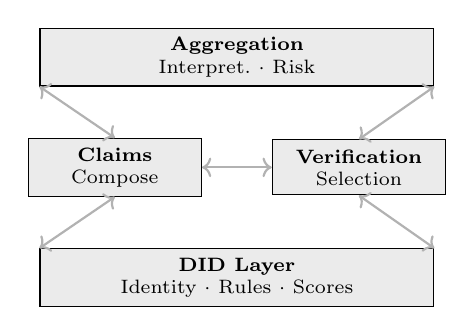
\begin{tikzpicture}[
    layer/.style={draw, minimum height=0.7cm, align=center, font=\scriptsize, fill=black!8},
    arr/.style={<->, thick, gray!60}
]
\node[layer, minimum width=5cm] (agg) at (0,2.8) {\textbf{Aggregation}\\Interpret.\ $\cdot$ Risk};
\node[layer, minimum width=2.2cm] (claim) at (-1.55,1.4) {\textbf{Claims}\\Compose};
\node[layer, minimum width=2.2cm] (verif) at (1.55,1.4) {\textbf{Verification}\\Selection};
\node[layer, minimum width=5cm] (did) at (0,0) {\textbf{DID Layer}\\Identity $\cdot$ Rules $\cdot$ Scores};

\draw[arr] (agg.south west) -- (claim.north);
\draw[arr] (agg.south east) -- (verif.north);
\draw[arr] (claim.east) -- (verif.west);
\draw[arr] (claim.south) -- (did.north west);
\draw[arr] (verif.south) -- (did.north east);
\end{tikzpicture}
\caption{RSN four-layer architecture.}
\label{fig:architecture}
\end{figure}

\subsection{Participant Roles}

A verification transaction involves up to six distinct DID roles (Fig.~\ref{fig:roles}): \textbf{Issuer} ($DID_I$, creates and submits the claim), \textbf{Subject} ($DID_S$, the DID the claim is about---may coincide with Issuer), \textbf{Authority} ($DID_A$, endorses the claim for a fee; may also offer witness services---\emph{optional}), \textbf{Witness} ($DID_{W_{1..n}}$, incognito monitor of verifier honesty via challenge codes---\emph{optional}), \textbf{Verifier} ($DID_V$, algorithmically selected to publish the claim), and the \textbf{RSN} (the network where verified claims are published). Any role may be delegated to another DID (Section~7.4). An Authority commonly bundles endorsement with witness services, but the two functions are logically independent.

\begin{figure}[ht]
\centering
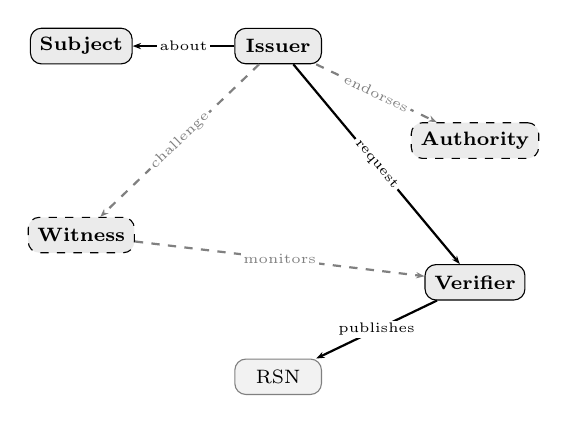
\begin{tikzpicture}[
    role/.style={draw, rounded corners, minimum width=1.1cm, minimum height=0.45cm, align=center, font=\scriptsize, fill=black!8},
    opt/.style={draw, rounded corners, minimum width=1.1cm, minimum height=0.45cm, align=center, font=\scriptsize, fill=black!8, dashed},
    arr/.style={-{Stealth[length=3pt]}, thick},
    oarr/.style={-{Stealth[length=3pt]}, thick, dashed, gray},
    lbl/.style={font=\tiny, fill=white, inner sep=1pt}
]
\node[role] (I) at (0,2.4) {\textbf{Issuer}};
\node[role] (S) at (-2.5,2.4) {\textbf{Subject}};
\node[opt] (A) at (2.5,1.2) {\textbf{Authority}};
\node[opt] (W) at (-2.5,0) {\textbf{Witness}};
\node[role] (V) at (2.5,-0.6) {\textbf{Verifier}};
\node[role, fill=black!5, draw=gray] (N) at (0,-1.8) {RSN};

\draw[arr] (I) -- node[lbl] {about} (S);
\draw[oarr] (I) -- node[lbl,sloped] {endorses} (A);
\draw[oarr] (I) -- node[lbl,sloped] {challenge} (W);
\draw[arr] (I) -- node[lbl,sloped] {request} (V);
\draw[oarr] (W) -- node[lbl] {monitors} (V);
\draw[arr] (V) -- node[lbl] {publishes} (N);
\end{tikzpicture}
\caption{DID roles in a verification transaction. Dashed = optional (Authority, Witness).}
\label{fig:roles}
\end{figure}

\subsection{Incorruptibility: Four Forces}

The incorruptibility of the RSN does not arise from a single mechanism but from four concurrent forces. None is sufficient on its own; only their combination makes an attempt at corruption economically irrational.

\textbf{Unpredictable target.} The verifier for each claim is selected non-deterministically through consistent hashing (Section~5.3). An attacker cannot pre-target a specific verifier for bribery, because the verifier's identity is a function of the claim's content and previous iterations, not of the issuer's choice.

\textbf{Reputational leverage---slow up, fast down.} Reputation can only be gained incrementally, through sustained consistent behavior. It can, however, be lost catastrophically in a single fraudulent endorsement (Section~6.2). This asymmetry means that years of accumulated reputation can be destroyed by one dishonest endorsement; the optimal strategy remains to reject suspicious claims.

\textbf{Public promise.} Every DID Holder publicly declares their policy---a machine-readable set of rules they commit to follow. Divergence between the declaration and actual behavior is detectable and priced as a reputational offense more severe than the underlying violation (Section~7.3). Hypocrisy is therefore costlier than direct dishonesty.

\textbf{Mesh attack-cost asymmetry.} The cost of censoring or destabilizing the network grows non-linearly with the network's size and density, while the cost of tolerating it remains constant. For censorship to pay off, a centralized actor would have to apply it across the entire network---requiring measures disproportionate to any conceivable benefit (Section~10).

% ============================================================
% 4. DECENTRALIZED IDENTITY MODEL
% ============================================================
\section{Decentralized Identity Model}

\subsection{DID with Special Properties}

The RSN extends the W3C DID Core specification~\cite{did2022} with: \textbf{Declared Rules} (machine-readable behavioral commitments), \textbf{Reputation Metadata} (aggregated behavioral score), and \textbf{Network Routing} (mutable onion gateway separate from the stable ring position).

\subsection{Claim Lifecycle}

A Claim proceeds through six stages (Fig.~\ref{fig:lifecycle}): composition, optional authority endorsement, verifier selection via consistent hashing, verification decision (accept or reject with iteration), publication, and reputation update for all parties.

\begin{figure}[ht]
\centering
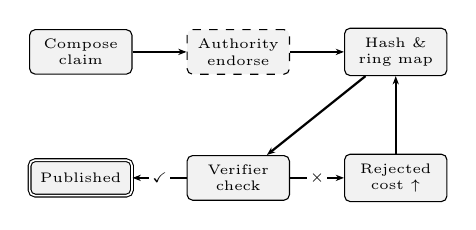
\begin{tikzpicture}[
    stp/.style={draw, rounded corners=2pt, minimum width=1.3cm, minimum height=0.45cm, align=center, font=\tiny, fill=black!5},
    arr/.style={-{Stealth[length=3pt]}, thick},
    lbl/.style={font=\tiny, fill=white, inner sep=1pt}
]
\node[stp] (comp) at (0,0) {Compose\\claim};
\node[stp, dashed] (auth) at (2.0,0) {Authority\\endorse};
\node[stp] (hash) at (4.0,0) {Hash \&\\ring map};
\node[stp] (ver) at (2.0,-1.6) {Verifier\\check};
\node[stp, double] (pub) at (0,-1.6) {Published};
\node[stp] (rej) at (4.0,-1.6) {Rejected\\cost $\uparrow$};

\draw[arr] (comp) -- (auth);
\draw[arr] (auth) -- (hash);
\draw[arr] (hash) -- (ver);
\draw[arr] (ver) -- node[lbl] {\checkmark} (pub);
\draw[arr] (ver) -- node[lbl] {$\times$} (rej);
\draw[arr] (rej) -- ++(0,0.8) -| (hash);
\end{tikzpicture}
\caption{Claim lifecycle with iteration loop.}
\label{fig:lifecycle}
\end{figure}

\subsection{Relationship to W3C DID Core}

The RSN's identity model is a proper superset of the W3C DID Core specification~\cite{did2022}. All RSN DIDs are valid W3C DIDs. The RSN-specific extensions are encoded as DID document properties defined in a dedicated DID method specification, compatible with existing infrastructure such as ION~\cite{buchner2021} and Ceramic~\cite{ceramic2023}.

% ============================================================
% 5. VERIFICATION AND PROPAGATION
% ============================================================
\section{Information Verification and Propagation}

\subsection{Cost of Information Entry}

The RSN's core economic principle is the asymmetry between reading and writing. Reading reputation data approaches zero marginal cost for participants who are part of the DID network and have access commensurate with their reputation---newcomers must gradually earn broader access (see anti-leeching). Writing---understood as the durable materialization of reputation into the network, not as a one-off technical act---requires verifiable cumulative investment across three dimensions: \textbf{time} (years of life spent on consistent behavior, fulfilled commitments, and cultivated relationships), \textbf{energy} (effort invested in honest dealing, care for partnerships, and long-term trustworthiness), and \textbf{money} (investment in one's own name---professional development, the quality of one's work, restitution for harms caused). Reputation cannot be purchased instantly---it is the outcome of lifelong accumulation that the system merely makes visible and transferable across contexts. The one-off technical costs of the protocol (cryptographic signatures, verifier fees) are negligible compared to this underlying investment.

\subsection{Social Graph and Contact Depth}

RSN is fundamentally a social network: each DID adds contacts (other DIDs) who permit the connection. These contacts have their own contacts, and so on. The algorithmic verifier search operates within a configurable depth $h$ of linked contacts (e.g., $h=3$: one's direct contacts, their contacts, and contacts of contacts). This architecture does not require a single global blockchain---it naturally favors the emergence of communities/clusters with overlaps into other communities. Every DID participant must have a published \textbf{policy}---a machine-readable set of rules governing how incoming requests are evaluated. Policy violations are recorded in the network as negative artifacts.

\subsection{Algorithmic Verifier Selection}

The verification protocol employs consistent hashing~\cite{karger1997} (Fig.~\ref{fig:verifier}). Verification is a paid service: verifiers operate for a fee, creating a market where competition drives pricing, speed, and reliability.

\textbf{Step 1.} The claim document is concatenated with the previous iteration's hash result (or $\varnothing$ on the first iteration) and hashed:
\begin{equation}
\text{pos} = f_h(\text{claim} \| \text{prev\_hash})
\label{eq:hash}
\end{equation}

The algorithm must include the \emph{complete path} of all previous requests and responses---not merely a hash of the previous iteration. Each verifier's full response (acceptance, rejection, quoted price, reason) is appended to the growing document, verifiable through cryptographic signatures at each step.

\textbf{Step 2.} The hash is mapped to $N$ positions on the consistent hash ring, evenly distributed (e.g., for $N=4$: $+0^{\circ}, +90^{\circ}, +180^{\circ}, +270^{\circ}$). From each position, a clockwise search selects the nearest DID as a verifier candidate (Fig.~\ref{fig:multipoint}). $N$ is a variable parameter that may depend on the percentage of currently active DIDs, time of day, or historical network responsiveness.

\textbf{Step 3.} The Verifier accepts (publishes, staking reputation) or rejects (returning to Step~1 with the rejection hash). When a node does not respond despite declaring online status, the next request must include all responses from all $N$ previous verifier candidates.

\textbf{Anti-leeching.} Target DIDs may set fees or access restrictions for queries from new DIDs with little reputation. This graduated mechanism (not binary) forces newcomers to build reputation through genuine activity before freely consuming others' data.

\begin{figure}[ht]
\centering
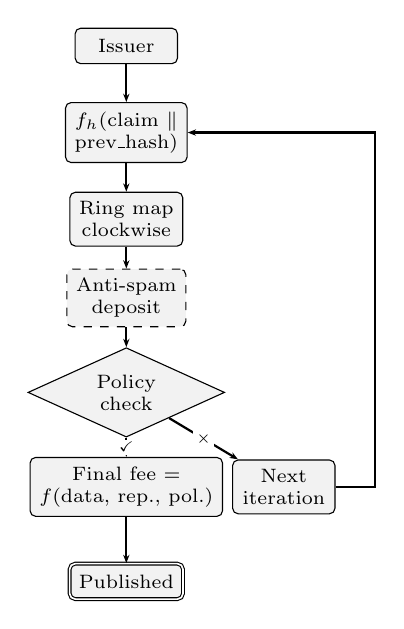
\begin{tikzpicture}[
    box/.style={draw, rounded corners=2pt, minimum width=1.3cm, minimum height=0.45cm, align=center, font=\scriptsize, fill=black!5},
    dec/.style={draw, diamond, aspect=2.2, minimum width=0.9cm, align=center, font=\scriptsize, fill=black!5},
    arr/.style={-{Stealth[length=3pt]}, thick},
    lbl/.style={font=\tiny, fill=white, inner sep=1pt}
]
\node[box] (iss) at (0,0) {Issuer};
\node[box] (hash) at (0,-1.1) {$f_h$(claim $\|$\\prev\_hash)};
\node[box] (ring) at (0,-2.2) {Ring map\\clockwise};
\node[box, dashed] (spam) at (0,-3.2) {Anti-spam\\deposit};
\node[dec] (check) at (0,-4.4) {Policy\\check};
\node[box] (rej) at (2,-5.6) {Next\\iteration};
\node[box] (fee) at (0,-5.6) {Final fee =\\$f$(data, rep., pol.)};
\node[box, double] (pub) at (0,-6.8) {Published};

\draw[arr] (iss) -- (hash);
\draw[arr] (hash) -- (ring);
\draw[arr] (ring) -- (spam);
\draw[arr] (spam) -- (check);
\draw[arr] (check) -- node[lbl] {$\times$} (rej);
\draw[arr] (check) -- node[lbl] {\checkmark} (fee);
\draw[arr] (fee) -- (pub);
\draw[arr] (rej.east) -- ++(0.5,0) |- (hash.east);
\end{tikzpicture}
\caption{Verifier selection protocol. Anti-spam deposit is optional and may be refundable. Final fee is paid only on acceptance.}
\label{fig:verifier}
\end{figure}

Each rejection appends the verifier's full response (including reasons and conditions) to the claim document, expanding its content. From the expanded document, a new hash is nondeterministically computed, mapping to a different ring position and selecting a different verifier. Documentation of the full path is mandatory---the issuer cannot predict or influence the next verifier. If a verifier ignores a request despite a compatible declared policy, witnesses (if present) record this, and the issuer may attach witness evidence upon final publication.

\begin{figure}[ht]
\centering
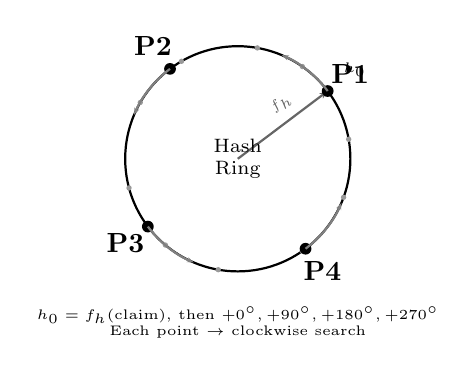
\begin{tikzpicture}[scale=0.65]
% Ring
\draw[thick] (0,0) circle (2.2cm);
% DID nodes on ring
\foreach \a in {10,55,80,120,150,195,230,260,305,340} {
  \fill[black!40] (\a:2.2) circle (1.5pt);
}
% Hash offset arrow pointing to initial position
\draw[-{Stealth[length=3pt]}, thick, black!60] (0,0) -- node[font=\tiny,above,sloped,pos=0.6] {$f_h$} (37:2.2);
\fill[black] (37:2.2) circle (2pt);
\node[font=\tiny,anchor=south west] at (37:2.35) {$h_0$};
% N=4 points offset from h0 by +0, +90, +180, +270
\foreach \offset/\l in {0/P1,90/P2,180/P3,270/P4} {
  \pgfmathsetmacro{\ang}{37+\offset}
  \node[fill=black, circle, inner sep=1.5pt] (p\offset) at (\ang:2.2) {};
  \node[font=\tiny,font=\bfseries] at (\ang:2.75) {\l};
  % clockwise search arc
  \draw[-{Stealth[length=2.5pt]}, thick, gray] (\ang:2.2) arc (\ang:\ang+30:2.2);
}
\node[font=\scriptsize, align=center] at (0,0) {Hash\\Ring};
\node[font=\tiny, align=center] at (0,-3.2) {$h_0 = f_h(\text{claim})$, then $+0^{\circ},+90^{\circ},+180^{\circ},+270^{\circ}$\\Each point $\rightarrow$ clockwise search};
\end{tikzpicture}
\caption{Multi-point selection ($N{=}4$). Hash $h_0$ sets the offset; 4 points evenly distributed from $h_0$.}
\label{fig:multipoint}
\end{figure}

\subsection{Witness Protocol}

The \textbf{Witness} role provides incognito accountability for verifier honesty through a cryptographic challenge-code protocol:

\textbf{Step W1.} The requester signs the verification request and sends it to $N_w$ witnesses---contacts from the requester's social network, or specialized witness-service providers operating for a fee.

\textbf{Step W2.} Each witness $w_i$ signs the entire signed request, retains the original signature $\sigma_i$, and computes a challenge code $c_i = h(\sigma_i)$. The challenge code is appended to the request.

\textbf{Step W3.} The request, now carrying $N_w$ challenge codes, is sent to the verifier. The verifier observes the codes but \emph{cannot determine} who the witnesses are or whether the codes correspond to real signatures.

\textbf{Step W4 (honest verifier).} If the verifier responds according to their declared policy, the challenge codes remain opaque. Witnesses are never revealed. No additional data is published.

\textbf{Step W5 (policy violation).} If the verifier violates their policy (ignores the request, responds inconsistently), the requester holds the witnesses' original signatures $\sigma_i$. These can be published as companion data: anyone can verify $c_i = h(\sigma_i)$, proving the witness was present. The requester can publish independently---the verifier already signed the challenge codes in their response.

\textbf{The bluff property.} The requester may substitute random values for some or all challenge codes. The verifier cannot distinguish genuine codes (backed by high-reputation authorities) from noise. This \emph{uncertainty} is the enforcement mechanism: every request carries the risk that a respected authority is watching incognito. The cost of maintaining this pressure is near zero (generating random numbers), while the potential cost of dishonesty for the verifier is catastrophic. Honest behavior is incentivized even in the absence of actual witnesses.

\textbf{Authority as witness.} An Authority that endorses a claim may bundle witness services: ``I endorse your claim and serve as incognito witness during verification.'' This is a natural business model---the Authority already has context. However, the two roles are logically independent.

\subsection{Expensive Radicalism Principle}

Three cost channels compound simultaneously (Fig.~\ref{fig:radicalism}):

\textbf{Channel 1: Iteration Cost.} Each rejection forces a new iteration consuming time and resources. Linear growth.

\textbf{Channel 2: Document Bloat.} Each iteration adds the full verifier response to the claim document. Growth is linear, but with a base offset: the initial payload (claim content, authority endorsement, cryptographic signatures) already has non-trivial size $B_0$. Total size after $k$ iterations: $S(k) = B_0 + k \cdot \Delta$, where $\Delta$ is the average response size.

\textbf{Channel 3: Verifier Risk Premium.} Risk is subjective. The verifier assesses whether the requesting DID's declared policies conflict with the verifier's own commercial, social, or political interests. The premium may escalate exponentially with perceived distance from the verifier's ``ideal'': $P(d) = \alpha \cdot e^{\beta d}$, where $d$ is the verifier's subjective distance metric. Beyond a personal no-go boundary, the verifier may refuse entirely.

\begin{figure}[ht]
\centering
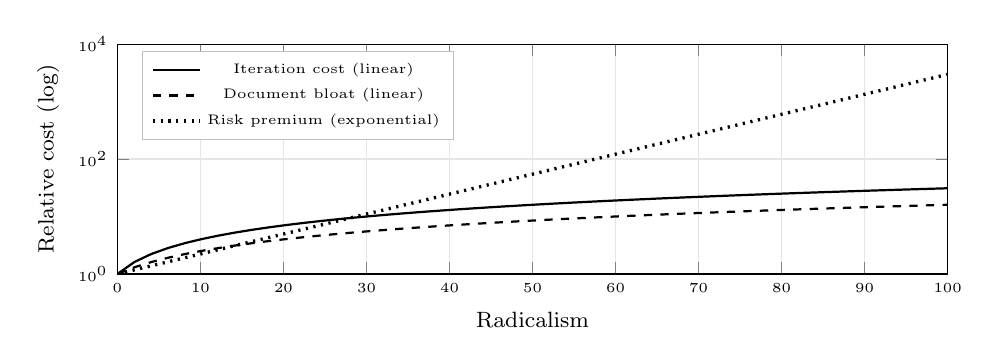
\begin{tikzpicture}
\begin{axis}[
    width=\columnwidth,
    height=4.5cm,
    xlabel={\footnotesize Radicalism},
    ylabel={\footnotesize Relative cost (log)},
    ymode=log,
    xmin=0, xmax=100,
    ymin=1, ymax=10000,
    grid=major,
    grid style={gray!20},
    legend style={at={(0.03,0.97)},anchor=north west,font=\tiny,draw=gray!50},
    tick label style={font=\tiny},
    label style={font=\footnotesize},
]
\addplot[black, thick, domain=0:100, samples=50] {1 + 0.3*x};
\addlegendentry{Iteration cost (linear)}
\addplot[black, thick, dashed, domain=0:100, samples=50] {1 + 0.15*x};
\addlegendentry{Document bloat (linear)}
\addplot[black, thick, dotted, line width=1.2pt, domain=0:100, samples=100] {exp(0.08*x)};
\addlegendentry{Risk premium (exponential)}
\end{axis}
\end{tikzpicture}
\caption{Cost escalation across three channels. The risk premium dominates at high radicalism.}
\label{fig:radicalism}
\end{figure}

Critically, this is not censorship. No claim is prohibited. The system prices risk (Table~\ref{tab:costs}).

\begin{table}[ht]
\centering
\caption{Cost comparison across claim types.}
\label{tab:costs}
\footnotesize
\begin{tabular}{@{}lcccc@{}}
\toprule
\textbf{Type} & \textbf{Iter.} & \textbf{Doc} & \textbf{Fee} & \textbf{Total} \\
\midrule
Credible & $k_{\min}$ & $B_0$ & $P_{\min}$ & Low \\
Controversial & $k_{\text{med}}$ & $B_0{+}k\Delta$ & $\alpha e^{\beta d}$ & Moderate \\
Radical & $k_{\max}$ & $\gg B_0$ & $\gg P_{\min}$ & Very high \\
Fraudulent & $\to\infty$ & --- & --- & Unpublishable \\
\bottomrule
\end{tabular}
\end{table}

% ============================================================
% 6. REPUTATION AND RISK
% ============================================================
\section{Reputation and Risk Assessment}

\subsection{Reputation Accumulation Model}

Reputation exhibits three properties: \textbf{slow accumulation} (incremental growth through consistent behavior), \textbf{rapid destruction} (a single fraud can reduce the score catastrophically), and \textbf{individual evaluation} (each consuming party may apply their own aggregation function).

\subsection{Reputable Authorities}

A Reputable Authority reviews claims and, if satisfied, co-signs them---staking its own reputation (Fig.~\ref{fig:authority}). The asymmetry is by design: gaining reputation is slow (incremental $+\delta$ per honest endorsement), while losing it is catastrophic ($-\Delta \gg \delta$ per false endorsement; illustratively, e.g., $+2\%$ vs.\ $-70\%$). The optimal strategy is always to reject suspicious claims. The specific values of $\delta$ and $\Delta$ are system parameters.

\begin{figure}[ht]
\centering
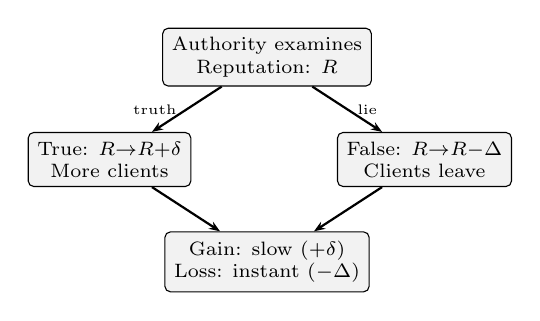
\begin{tikzpicture}[
    box/.style={draw, rounded corners=2pt, minimum width=2cm, minimum height=0.6cm, align=center, font=\scriptsize, fill=black!5},
    arr/.style={-{Stealth[length=4pt]}, thick}
]
\node[box] (exam) at (0,0) {Authority examines\\Reputation: $R$};
\node[box] (true) at (-2,-1.3) {True: $R{\to}R{+}\delta$\\More clients};
\node[box] (false) at (2,-1.3) {False: $R{\to}R{-}\Delta$\\Clients leave};
\node[box] (insight) at (0,-2.6) {Gain: slow ($+\delta$)\\Loss: instant ($-\Delta$)};

\draw[arr] (exam) -- node[left,font=\tiny] {truth} (true);
\draw[arr] (exam) -- node[right,font=\tiny] {lie} (false);
\draw[arr] (true) -- (insight);
\draw[arr] (false) -- (insight);
\end{tikzpicture}
\caption{Reputable Authority---asymmetric incentives.}
\label{fig:authority}
\end{figure}

\subsection{Multi-Dimensional Reputation}

Reputation is not a scalar but a vector across multiple dimensions: financial reliability, personal integrity, professional competence, civic engagement, and others (Fig.~\ref{fig:reputation-radar}). Different evaluation providers project this vector differently depending on context---a lender prioritizes financial reliability, an employer professional competence, a neighbor civic behavior. There is no single ``correct'' reputation score; only perspectives.

\begin{figure}[ht]
\centering
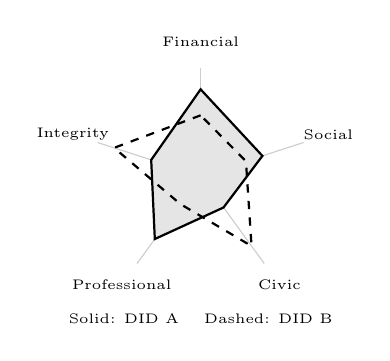
\begin{tikzpicture}[scale=0.55]
\foreach \a/\l in {90/Financial,162/Integrity,234/Professional,306/Civic,18/Social} {
  \draw[gray!40] (0,0) -- (\a:2.5);
  \node[font=\tiny, align=center] at (\a:3.1) {\l};
  \foreach \r in {0.8,1.6,2.4} {
    \fill[black!15] (\a:\r) circle (0.5pt);
  }
}
\draw[thick, fill=black!10] (90:2.0) -- (162:1.2) -- (234:1.8) -- (306:0.9) -- (18:1.5) -- cycle;
\draw[thick, dashed] (90:1.4) -- (162:2.1) -- (234:0.8) -- (306:2.0) -- (18:1.1) -- cycle;
\node[font=\tiny] at (0,-3.3) {Solid: DID A \quad Dashed: DID B};
\end{tikzpicture}
\caption{Multi-dimensional reputation vectors. Different DIDs exhibit different profiles across dimensions.}
\label{fig:reputation-radar}
\end{figure}

\subsection{Democratized Risk Assessment}

The RSN democratizes systematic risk assessment---a capability currently concentrated in financial institutions but applicable far beyond banking. Industrial conglomerates assessing supplier reliability, insurance companies pricing behavioral risk, due diligence for mergers and acquisitions, equipment lifetime estimation in manufacturing---anywhere counterparty risk requires assessment, the RSN provides a decentralized, market-driven alternative. A market of interpretation services translates raw multi-dimensional reputation data into actionable summaries, making counterparty evaluation accessible to any participant at marginal cost.

% ============================================================
% 7. CONSENSUS AND DISPUTE RESOLUTION
% ============================================================
\section{Consensus and Dispute Resolution}

\subsection{Decentralized Justice Model}

The RSN reframes justice as a bilateral negotiation problem. The threat of permanent, verifiable reputation damage is a more effective deterrent than legal proceedings the harmed party cannot afford.

\subsection{Emergent Consensus}

Each participant maintains a personal satisfaction threshold. The network's aggregate consensus emerges as the statistical average of thousands of bilateral negotiations (Fig.~\ref{fig:consensus}). A response far above the consensus (barbaric) is expensive to publish. A response near the consensus (proportional) is cheap. The consensus is not a rule---it is a price signal.

\begin{figure}[ht]
\centering
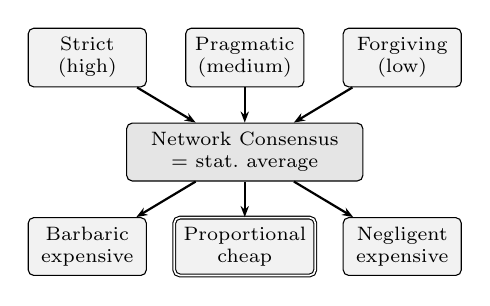
\begin{tikzpicture}[
    person/.style={draw, rounded corners=2pt, minimum width=1.5cm, minimum height=0.5cm, align=center, font=\scriptsize, fill=black!5},
    arr/.style={-{Stealth[length=4pt]}, thick}
]
\node[person] (a) at (-2,0) {Strict\\(high)};
\node[person] (b) at (0,0) {Pragmatic\\(medium)};
\node[person] (c) at (2,0) {Forgiving\\(low)};
\node[person, fill=black!10, minimum width=3cm] (cons) at (0,-1.2) {Network Consensus\\= stat.\ average};
\node[person] (exp) at (-2,-2.4) {Barbaric\\expensive};
\node[person, double] (prop) at (0,-2.4) {Proportional\\cheap};
\node[person] (neg) at (2,-2.4) {Negligent\\expensive};

\draw[arr] (a) -- (cons);
\draw[arr] (b) -- (cons);
\draw[arr] (c) -- (cons);
\draw[arr] (cons) -- (exp);
\draw[arr] (cons) -- (prop);
\draw[arr] (cons) -- (neg);
\end{tikzpicture}
\caption{Emergent consensus from individual satisfaction thresholds.}
\label{fig:consensus}
\end{figure}

\subsection{Punishment Calibration}

Each DID Holder publicly declares responses to specific misconduct categories. Disproportionately harsh or lenient declarations attract negative reputation signals. Proportional declarations are accepted without friction---a self-calibrating punishment system.

Consensus declarations are themselves subject to hypocrisy detection: declaratively committing to a consensus position while behaving inconsistently constitutes a reputational offense more severe than the underlying deviation, as it demonstrates intentional deception.

\subsection{Delegation}

All activities within a DID---with one exception---may be delegated to another DID. \textbf{The Subject role---the DID whose behavior the claim is about---cannot be delegated; it is non-transferably bound to the identity holder to whom the claim refers.} The other active roles---Issuer, Authority, Witness, Verifier---can be transferred to a designated delegate DID, whether for verification, claim submission, consensus participation, or dispute resolution. Delegation is revocable at any time. This enables specialization (e.g., professional verification services) while the Holder retains ultimate control and responsibility. Delegation applies across the entire system and is essential for scalability.

\subsection{From Individual Morality to Emergent Social Contract}

Each DID's declared policy represents a formalization of individual morality: what the Holder considers acceptable, how they respond to specific behaviors, what they require from counterparties. These policies are not imposed by a system designer---they are chosen by each participant and expressed in machine-readable form.

This formalization enables a three-stage emergence. First, individual morality is encoded as \textbf{policy}---a set of declared rules, thresholds, and response functions that the DID commits to follow. Second, the aggregate of all policies across the network produces \textbf{emergent ethics}---statistically observable norms that no single participant designed but that arise from the interaction of thousands of individual moral positions~\cite{durkheim1893}. Third, these emergent ethics, expressed as shared behavioral norms enforced through bilateral price signals, constitute a \textbf{measurable social contract}---not a theoretical construct that nobody signed~\cite{rawls1971}, but an empirically observable set of rules backed by actual behavior.

This process mirrors findings from moral foundations theory~\cite{haidt2012}: human morality is intuitive, pluralistic, and culturally variable. The RSN does not require moral consensus as an input; it produces behavioral consensus as an output. The resulting social contract is not static---it evolves as participants join, leave, and adjust their policies in response to network feedback. Unlike classical social contract theory, this contract is revocable, observable, and enforceable without a sovereign.

% ============================================================
% 8. ECONOMIC MODEL
% ============================================================
\section{Economic Model}

The preceding sections described a tool---the RSN's verification mechanisms, cost structure, and emergent consensus. This section describes a methodology for applying this tool to fiscal and governance transition. The tool is general-purpose; the methodology below is one possible application.

\subsection{Incentive Structure}

Reputation as capital creates direct incentives for honest behavior. In normal operation, participants build reputation naturally through everyday transactions and fulfilled commitments. The primary expenditure is on \emph{negative} claims---recording harm done by others. This asymmetry incentivizes useful, reliable behavior: being honest costs nothing extra, while being harmful creates a documented trail that others will pay to preserve. Hypocrisy---declaring rules without following them---is the most expensive failure mode, as it demonstrates intentional deception.

\subsection{Parallel Fiscal System}

Three components enable competitive pressure: (1)~\textbf{Simple Tax}---a single proportional rate with no exceptions, initially marginally below the existing effective rate; (2)~\textbf{Electronic Spending Registration (ESR)}---inverting the Czech EET model so citizens surveil state expenditures; (3)~\textbf{Citizen-Directed Tax Allocation}---starting at a few percent in the first year and reaching, after a decade, anywhere from the low double digits to a full migration to a citizen-directed system, depending on the rate of adoption. The actual tempo depends on the speed at which free-market alternatives to state services emerge and on the state's willingness to cooperate with the transition; the function of time need not be linear, and there is no reason to set an upper bound on where adoption may ultimately arrive.

% ============================================================
% 9. MIGRATION PATH
% ============================================================
\section{Migration Path}

The migration proceeds through three phases (Fig.~\ref{fig:migration}): \textbf{Phase~1: Overlay} (RSN as informational layer, state is sole provider), \textbf{Phase~2: Competition} (RSN provides functional alternatives, dual-system use), and \textbf{Phase~3: Transition} (RSN outperforms state equivalents, voluntary migration). The transition is reversible at every stage.

\begin{figure}[ht]
\centering
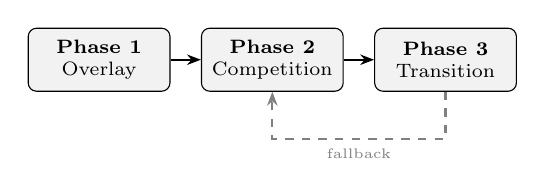
\begin{tikzpicture}[
    phase/.style={draw, rounded corners=3pt, minimum width=1.8cm, minimum height=0.8cm, align=center, font=\scriptsize, fill=black!5},
    arr/.style={-{Stealth[length=5pt]}, thick}
]
\node[phase] (p1) at (0,0) {\textbf{Phase 1}\\Overlay};
\node[phase] (p2) at (2.2,0) {\textbf{Phase 2}\\Competition};
\node[phase] (p3) at (4.4,0) {\textbf{Phase 3}\\Transition};

\draw[arr] (p1) -- (p2);
\draw[arr] (p2) -- (p3);
\draw[arr, dashed, gray] (p3.south) -- ++(0,-0.6) -| node[below,font=\tiny,pos=0.25] {fallback} (p2.south);
\end{tikzpicture}
\caption{Three-phase migration---reversible at every stage.}
\label{fig:migration}
\end{figure}

The primary pressure mechanism is fiscal: when conditional taxpayers reach an ``economically significant minority $X$''---a group large enough that repression against it causes non-trivial economic damage and civil disobedience becomes a credible threat---the state enters negotiation. For illustration, we use $X \approx 15\%$ of GDP, but the actual threshold depends on the specific economy.

% ============================================================
% 10. SECURITY ANALYSIS
% ============================================================
\section{Security Analysis}

We consider five adversary categories: individual bad actors, organized groups, corporate adversaries, state-level adversaries, and protocol-level adversaries.

\textbf{Sybil resistance}~\cite{douceur2002}. Building reputation requires sustained, verifiable interaction. The cost of a successful Sybil attack scales linearly with fake identities and quadratically with the target reputation level. Operating multiple DIDs in parallel is possible but expensive by design---each identity must independently accumulate reputation through genuine activity. In free societies this cost deters casual abuse; in dictatorships, parallel DIDs become a survival tool enabling compartmentalized resistance, underground coordination, and safer black-market navigation.

\textbf{Collusion defense.} Patterns of mutual endorsement among closed groups are detectable through social graph analysis. Reputation aggregation functions discount claims from tightly clustered sources.

\textbf{State-level adversary.} Onion routing, absence of centralized infrastructure, and distribution of the Verifier role across the participant base ensure that suppression requires measures disproportionate to any benefit.

\textbf{Privacy vs.\ accountability.} Pseudonymity---a middle ground between anonymity and identity disclosure---allows DIDs to accumulate meaningful reputation without revealing the Holder's real-world identity.

% ============================================================
% 11. PRIVACY
% ============================================================
\section{Privacy Considerations}

The RSN's privacy model is built on pseudonymity. The Holder controls identity disclosure: minimal (pure pseudonym), selective (specific credentials linked), or full (legal identity associated). Published claims are permanent---the system supports contextual correction but not erasure. A Holder may abandon a compromised DID and start anew, forfeiting accumulated reputation.

% ============================================================
% 12. RELATED WORK
% ============================================================
\section{Related Work}

The W3C DID Core specification~\cite{did2022} and Ceramic Network~\cite{ceramic2023} provide the identity foundation. EigenTrust~\cite{kamvar2003} demonstrated distributed reputation aggregation without central authority. SBTs~\cite{weyl2022} introduced non-transferable social tokens. The RSN differs in its emphasis on economic cost as a quality filter and its mechanism for pricing radicalism.

DAOs~\cite{buterin2014} and quadratic voting~\cite{buterin2019} demonstrated feasibility of decentralized governance. The RSN derives consensus from bilateral price negotiations rather than voting.

The proposal draws on anarcho-capitalist theory~\cite{rothbard1973,hoppe2001} for private service provision but departs in two critical respects: it designs for spite and retributive impulses rather than assuming rationality, and it proposes gradual transition rather than revolution. The concept of emergent social contracts has antecedents in Hayek's theory of spontaneous order~\cite{hayek1973}.

\textbf{Anarcho-agorism.} The RSN shares significant common ground with agorist counter-economics~\cite{konkin2006}---particularly the emphasis on building parallel institutions and voluntary exchange. However, agorism tends to assume rational self-interest as a sufficient coordination mechanism and often lacks a concrete migration path from existing state structures. The RSN explicitly incorporates non-rational behavioral tendencies and provides a fiscal pressure mechanism for gradual transition.

\textbf{Meritocracy.} The RSN may represent a first functional description of how meritocracy~\cite{young1958} can emerge as a systemic property rather than a slogan. Traditional meritocratic systems fail because they require a central authority to define and enforce ``merit.'' In the RSN, merit emerges from bilateral evaluations: those who deliver value accumulate reputation; no committee decides who has merit.

\textbf{Property as privilege.} The RSN departs fundamentally from anarcho-capitalist and Austrian-school treatments of property rights as natural and absolute. In the RSN framework, property is a \emph{privilege}---a social recognition that can, in extreme cases, be withdrawn by the community when a participant fundamentally violates shared norms (betrayal, refusal to defend the community in existential crisis, systematic exploitation). This is not state expropriation but a withdrawal of social recognition by the network of bilateral relationships.

% ============================================================
% 13. LIMITATIONS
% ============================================================
\section{Discussion and Limitations}

\textbf{Cold start.} The RSN's value depends on network effects; early adopters face limited value until participation reaches a threshold. However, even from early stages, the DID network serves as a useful supplementary information source. Early reputation evaluation and authority assessment are expected to develop gradually with increasing sophistication.

\textbf{Anti-leeching and access control.} Target DIDs may impose graduated fees and access restrictions on queries from low-reputation DIDs. This is not binary but a continuous scale: the less reputation a querying DID has, the less information it receives, the longer it waits, and the more it pays. This mechanism incentivizes genuine participation over passive consumption.

\textbf{Inequality of access.} The cost of publishing claims may filter legitimate grievances from economically disadvantaged participants. Mitigation: every participant simultaneously serves as a potential verifier (or delegates this role) and earns verification fees. Over a sufficient time horizon, a non-radical participant should approach financial neutrality---verification income approximately offsetting publication costs. This is a statistical expectation, not a guarantee.

\textbf{Reputation inequality.} Early adopters accumulate advantages that may create barriers for latecomers. However, reputation evaluation is performed by third-party providers who may choose to mitigate first-mover advantage through their aggregation algorithms. Being first with a good reputation is a legitimate comparative economic advantage---and that is by design.

\textbf{Open questions.} Optimal cost functions, aggregation standards, protocol governance, and interaction with AI-generated synthetic reputation data remain areas for future work.

This paper does not claim that the RSN will produce optimal outcomes in all circumstances. It claims that the RSN represents a \emph{feasible} alternative---technically implementable, economically self-sustaining, and socially compatible with human behavioral tendencies as they actually are.

% ============================================================
% 14. CONCLUSION
% ============================================================
\section{Conclusion}

This paper has presented the Reputation Social Network, a decentralized protocol enabling pseudonymous, verifiable reputation exchange. The Expensive Radicalism Principle ensures that fraudulent claims are priced out without censorship. The proposed migration path enables gradual, reversible transition from existing institutions. The design incorporates human nature as it is---including pettiness, spite, and the desire for retributive satisfaction---rather than requiring ideological transformation. The result is not utopia but a system where justice is accessible, reputation is earned, and the cost of misconduct is borne by the party who caused it.

% ============================================================
% REFERENCES
% ============================================================
\bibliography{references}

\end{document}
